\chapter{Arquitetura funcional}


\begin{figure}[h]
    \centering
    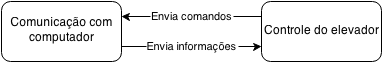
\includegraphics[width=0.8\columnwidth]{./figures/arq_funcional.png}
    \caption{Diagrama de blocos da arquitetura funcional do sistema.}
    \label{fig:arq_funcional}
\end{figure}


Cada uma das funções envolve as seguintes subpartes:

\begin{enumerate}
	\item Comunicação com computador
	\begin{enumerate}
		\item $<<$ISR$>>$ Comunicação
		\begin{enumerate}
			\item Efetua o gerenciamento da UART;
			\item Possui filas FIFO de recebimento e envio de dados;
			\item Provê ao sistema uma camada de abstração para comunicação bidirecional com o elevador (que é simulado no compuador).
		\end{enumerate}
	\end{enumerate}
	
	\item Controle do elevador
	\begin{enumerate}
		\item $<<$Ativo$>>$ Controlador do elevador
		\begin{enumerate}
			\item Acende um botão assim que um usuário o pressiona;
			\item Atende a requisições para todos os andares;
			\item Toma decisões e envia comandos para os atuadores do elevador;
			\item Possui dois estados de movimento bem definidos para o elevador: subida e descida.
% 			\item Possui um vetor que indica quais requisições de botões estão pendentes.
		\end{enumerate}
		\item $<<$Passivo$>>$ Protocolo de comunicação
		\begin{enumerate}
			\item Recebe requisições de botões de andares do elevador;
			\item Envia comandos de acender/apagar luzes dos botões do elevador;
			\item Envia comandos de abrir/fechar portas ao elevador;
			\item Envia comandos de subida/descida ao elevador.
		\end{enumerate}
	\end{enumerate}
\end{enumerate}


\section{Alocação das funções em Hardware e Software}

A função de comunicação com o computador constitui-se tanto de hardware quanto de software. A parte de hardware está relacionada ao periférico UART0 do Kit LPC1768. O software relaciona-se ao driver desenvolvido para inicializar e utilizar este periférico.

A função de controle do elevador é constituída apenas de software, uma vez que constitui-se do programa a ser desenvolvido para controlar a lógica de operação do elevador.




